% Options for packages loaded elsewhere
\PassOptionsToPackage{unicode}{hyperref}
\PassOptionsToPackage{hyphens}{url}
%
\documentclass[
]{article}
\usepackage{amsmath,amssymb}
\usepackage{iftex}
\ifPDFTeX
  \usepackage[T1]{fontenc}
  \usepackage[utf8]{inputenc}
  \usepackage{textcomp} % provide euro and other symbols
\else % if luatex or xetex
  \usepackage{unicode-math} % this also loads fontspec
  \defaultfontfeatures{Scale=MatchLowercase}
  \defaultfontfeatures[\rmfamily]{Ligatures=TeX,Scale=1}
\fi
\usepackage{lmodern}
\ifPDFTeX\else
  % xetex/luatex font selection
\fi
% Use upquote if available, for straight quotes in verbatim environments
\IfFileExists{upquote.sty}{\usepackage{upquote}}{}
\IfFileExists{microtype.sty}{% use microtype if available
  \usepackage[]{microtype}
  \UseMicrotypeSet[protrusion]{basicmath} % disable protrusion for tt fonts
}{}
\makeatletter
\@ifundefined{KOMAClassName}{% if non-KOMA class
  \IfFileExists{parskip.sty}{%
    \usepackage{parskip}
  }{% else
    \setlength{\parindent}{0pt}
    \setlength{\parskip}{6pt plus 2pt minus 1pt}}
}{% if KOMA class
  \KOMAoptions{parskip=half}}
\makeatother
\usepackage{xcolor}
\usepackage[margin=1in]{geometry}
\usepackage{color}
\usepackage{fancyvrb}
\newcommand{\VerbBar}{|}
\newcommand{\VERB}{\Verb[commandchars=\\\{\}]}
\DefineVerbatimEnvironment{Highlighting}{Verbatim}{commandchars=\\\{\}}
% Add ',fontsize=\small' for more characters per line
\usepackage{framed}
\definecolor{shadecolor}{RGB}{248,248,248}
\newenvironment{Shaded}{\begin{snugshade}}{\end{snugshade}}
\newcommand{\AlertTok}[1]{\textcolor[rgb]{0.94,0.16,0.16}{#1}}
\newcommand{\AnnotationTok}[1]{\textcolor[rgb]{0.56,0.35,0.01}{\textbf{\textit{#1}}}}
\newcommand{\AttributeTok}[1]{\textcolor[rgb]{0.13,0.29,0.53}{#1}}
\newcommand{\BaseNTok}[1]{\textcolor[rgb]{0.00,0.00,0.81}{#1}}
\newcommand{\BuiltInTok}[1]{#1}
\newcommand{\CharTok}[1]{\textcolor[rgb]{0.31,0.60,0.02}{#1}}
\newcommand{\CommentTok}[1]{\textcolor[rgb]{0.56,0.35,0.01}{\textit{#1}}}
\newcommand{\CommentVarTok}[1]{\textcolor[rgb]{0.56,0.35,0.01}{\textbf{\textit{#1}}}}
\newcommand{\ConstantTok}[1]{\textcolor[rgb]{0.56,0.35,0.01}{#1}}
\newcommand{\ControlFlowTok}[1]{\textcolor[rgb]{0.13,0.29,0.53}{\textbf{#1}}}
\newcommand{\DataTypeTok}[1]{\textcolor[rgb]{0.13,0.29,0.53}{#1}}
\newcommand{\DecValTok}[1]{\textcolor[rgb]{0.00,0.00,0.81}{#1}}
\newcommand{\DocumentationTok}[1]{\textcolor[rgb]{0.56,0.35,0.01}{\textbf{\textit{#1}}}}
\newcommand{\ErrorTok}[1]{\textcolor[rgb]{0.64,0.00,0.00}{\textbf{#1}}}
\newcommand{\ExtensionTok}[1]{#1}
\newcommand{\FloatTok}[1]{\textcolor[rgb]{0.00,0.00,0.81}{#1}}
\newcommand{\FunctionTok}[1]{\textcolor[rgb]{0.13,0.29,0.53}{\textbf{#1}}}
\newcommand{\ImportTok}[1]{#1}
\newcommand{\InformationTok}[1]{\textcolor[rgb]{0.56,0.35,0.01}{\textbf{\textit{#1}}}}
\newcommand{\KeywordTok}[1]{\textcolor[rgb]{0.13,0.29,0.53}{\textbf{#1}}}
\newcommand{\NormalTok}[1]{#1}
\newcommand{\OperatorTok}[1]{\textcolor[rgb]{0.81,0.36,0.00}{\textbf{#1}}}
\newcommand{\OtherTok}[1]{\textcolor[rgb]{0.56,0.35,0.01}{#1}}
\newcommand{\PreprocessorTok}[1]{\textcolor[rgb]{0.56,0.35,0.01}{\textit{#1}}}
\newcommand{\RegionMarkerTok}[1]{#1}
\newcommand{\SpecialCharTok}[1]{\textcolor[rgb]{0.81,0.36,0.00}{\textbf{#1}}}
\newcommand{\SpecialStringTok}[1]{\textcolor[rgb]{0.31,0.60,0.02}{#1}}
\newcommand{\StringTok}[1]{\textcolor[rgb]{0.31,0.60,0.02}{#1}}
\newcommand{\VariableTok}[1]{\textcolor[rgb]{0.00,0.00,0.00}{#1}}
\newcommand{\VerbatimStringTok}[1]{\textcolor[rgb]{0.31,0.60,0.02}{#1}}
\newcommand{\WarningTok}[1]{\textcolor[rgb]{0.56,0.35,0.01}{\textbf{\textit{#1}}}}
\usepackage{graphicx}
\makeatletter
\def\maxwidth{\ifdim\Gin@nat@width>\linewidth\linewidth\else\Gin@nat@width\fi}
\def\maxheight{\ifdim\Gin@nat@height>\textheight\textheight\else\Gin@nat@height\fi}
\makeatother
% Scale images if necessary, so that they will not overflow the page
% margins by default, and it is still possible to overwrite the defaults
% using explicit options in \includegraphics[width, height, ...]{}
\setkeys{Gin}{width=\maxwidth,height=\maxheight,keepaspectratio}
% Set default figure placement to htbp
\makeatletter
\def\fps@figure{htbp}
\makeatother
\setlength{\emergencystretch}{3em} % prevent overfull lines
\providecommand{\tightlist}{%
  \setlength{\itemsep}{0pt}\setlength{\parskip}{0pt}}
\setcounter{secnumdepth}{-\maxdimen} % remove section numbering
\ifLuaTeX
  \usepackage{selnolig}  % disable illegal ligatures
\fi
\IfFileExists{bookmark.sty}{\usepackage{bookmark}}{\usepackage{hyperref}}
\IfFileExists{xurl.sty}{\usepackage{xurl}}{} % add URL line breaks if available
\urlstyle{same}
\hypersetup{
  pdftitle={Parkinson data - II},
  pdfauthor={Giovanni Saraceno},
  hidelinks,
  pdfcreator={LaTeX via pandoc}}

\title{Parkinson data - II}
\author{Giovanni Saraceno}
\date{}

\begin{document}
\maketitle

{
\setcounter{tocdepth}{2}
\tableofcontents
}
\begin{Shaded}
\begin{Highlighting}[]
\FunctionTok{library}\NormalTok{(tidyverse)}
\FunctionTok{library}\NormalTok{(dplyr)}
\FunctionTok{library}\NormalTok{(ggplot2)}
\end{Highlighting}
\end{Shaded}

\begin{Shaded}
\begin{Highlighting}[]
\NormalTok{dat }\OtherTok{\textless{}{-}} \FunctionTok{read.csv}\NormalTok{(}\StringTok{\textquotesingle{}parkinsons\_updrs.data\textquotesingle{}}\NormalTok{, }\AttributeTok{he =} \ConstantTok{TRUE}\NormalTok{, }\AttributeTok{sep =} \StringTok{\textquotesingle{},\textquotesingle{}}\NormalTok{)}
\NormalTok{dat}\SpecialCharTok{$}\NormalTok{subject. }\OtherTok{\textless{}{-}} \FunctionTok{as.factor}\NormalTok{(dat}\SpecialCharTok{$}\NormalTok{subject.)}
\NormalTok{dat}\SpecialCharTok{$}\NormalTok{sex }\OtherTok{\textless{}{-}} \FunctionTok{ifelse}\NormalTok{(dat}\SpecialCharTok{$}\NormalTok{sex }\SpecialCharTok{==} \DecValTok{1}\NormalTok{, }\StringTok{\textquotesingle{}F\textquotesingle{}}\NormalTok{, }\StringTok{\textquotesingle{}M\textquotesingle{}}\NormalTok{)}
\NormalTok{dat}\SpecialCharTok{$}\NormalTok{sex }\OtherTok{\textless{}{-}} \FunctionTok{as.factor}\NormalTok{(dat}\SpecialCharTok{$}\NormalTok{sex)}
\end{Highlighting}
\end{Shaded}

\hypertarget{multiple-linear-regression}{%
\paragraph{Multiple Linear
Regression}\label{multiple-linear-regression}}

Suppose that data consist of \(\{y_i, \mathbf{x}_i\}\), where each
observation consists of a scalr response \(y_i\) and a vector of
\(\mathbf{x}_i\) (covariates) of \(p\) parameter regressors. In the
multiple linear regression model we have
\[y_i = \beta_1 x_{i1} + \beta_2 x_{i2} + \ldots + \beta_p x_{ip} - \epsilon_i\]
or equivalently
\[\mathbf{y} = \mathbf{X} \mathbf{\beta} + \mathbf{\epsilon},\] where
\(\mathbf{y}\) and \(\mathbf{\epsilon}\) are \(n \times 1\) vectors of
the response variables and the errors of the \(n\) observations, and
\(\mathbf{X}\) is an \(n \times p\) matrix of regressors, also sometimes
called the design matrix, whose row \(i\) contains the \(i\)-th
observations on all the explanatory variables.

In order to estimates the \(\beta\)'s parameters, the most famous method
id the ordinary least squares (OLS). It is based on minimizing the sum
of squared residuals.

It is common to assess the goodness-of-fit of the OLS regression by
comparing how much the initial variation in the sample can be reduced by
regressing onto X. The coefficient of determination \(R^2\) is defined
as a ratio of ``explained'' variance to the ``total'' variance of the
dependent variable \(y\), in the cases where the regression sum of
squares equals the sum of squares of residuals
\[R^2 = \frac{\sum(\hat{y}_i - \bar{y})^2}{\sum(y_i - \bar{y})^2} = 1 - \frac{RSS}{TSS}\]
where TSS is the total sum of squares for the dependent variable. In
order for \(R^2\) to be meaningful, the matrix \(X\) of data on
regressors must contain a column vector of ones to represent the
constant whose coefficient is the regression intercept. In that case,
\(R^2\) will always be a number between 0 and 1, with values close to 1
indicating a good degree of fit.

Let's see the application to the Parkinson data.

\begin{Shaded}
\begin{Highlighting}[]
\NormalTok{mod1 }\OtherTok{\textless{}{-}} \FunctionTok{lm}\NormalTok{(total\_UPDRS }\SpecialCharTok{\textasciitilde{}}\NormalTok{ age }\SpecialCharTok{+}\NormalTok{ sex }\SpecialCharTok{+}\NormalTok{ test\_time }\SpecialCharTok{+}\NormalTok{ Jitter... }\SpecialCharTok{+}
\NormalTok{             Shimmer }\SpecialCharTok{+}\NormalTok{ NHR }\SpecialCharTok{+}\NormalTok{ HNR }\SpecialCharTok{+}\NormalTok{ RPDE }\SpecialCharTok{+}\NormalTok{ DFA }\SpecialCharTok{+}\NormalTok{ PPE,}
           \AttributeTok{data =}\NormalTok{ dat)}
\FunctionTok{summary}\NormalTok{(mod1)}
\end{Highlighting}
\end{Shaded}

\begin{verbatim}
## 
## Call:
## lm(formula = total_UPDRS ~ age + sex + test_time + Jitter... + 
##     Shimmer + NHR + HNR + RPDE + DFA + PPE, data = dat)
## 
## Residuals:
##     Min      1Q  Median      3Q     Max 
## -27.970  -7.473  -1.578   7.343  26.858 
## 
## Coefficients:
##               Estimate Std. Error t value Pr(>|t|)    
## (Intercept)  37.993036   3.090434  12.294  < 2e-16 ***
## age           0.309125   0.015065  20.520  < 2e-16 ***
## sexM          1.895360   0.293151   6.465 1.09e-10 ***
## test_time     0.015600   0.002397   6.508 8.27e-11 ***
## Jitter...   101.443427  50.074953   2.026   0.0428 *  
## Shimmer     -42.262092  10.186302  -4.149 3.39e-05 ***
## NHR         -22.390765   5.137487  -4.358 1.33e-05 ***
## HNR          -0.587395   0.067702  -8.676  < 2e-16 ***
## RPDE          3.083135   1.754558   1.757   0.0789 .  
## DFA         -33.414836   2.220918 -15.046  < 2e-16 ***
## PPE          12.193496   2.609037   4.674 3.03e-06 ***
## ---
## Signif. codes:  0 '***' 0.001 '**' 0.01 '*' 0.05 '.' 0.1 ' ' 1
## 
## Residual standard error: 9.792 on 5864 degrees of freedom
## Multiple R-squared:  0.164,  Adjusted R-squared:  0.1626 
## F-statistic:   115 on 10 and 5864 DF,  p-value: < 2.2e-16
\end{verbatim}

The output of a linear model includes:

\begin{enumerate}
\def\labelenumi{\arabic{enumi}.}
\tightlist
\item
  \textbf{Std. Error} is the standard deviation of the sampling
  distribution of the estimate of the coefficient under the standard
  regression assumptions. Such standard deviations are called standard
  errors of the corresponding quantity (the coefficient estimate in this
  case).
\item
  \textbf{t value} is the value of the t-statistic for testing whether
  the corresponding regression coefficient is different from 0.
\item
  \textbf{Pr.} is the p-value for the hypothesis test for which the t
  value is the test statistic. It tells you the probability of a test
  statistic at least as unusual as the one you obtained, if the null
  hypothesis were true. In this case, the null hypothesis is that the
  true coefficient is zero; if that probability is low, it's suggesting
  that it would be rare to get a result as unusual as this if the
  coefficient were really zero.
\item
  The \textbf{Residual standard error} represents the standard deviation
  of the residuals. It's a measure of how close the fit is to the
  points.
\item
  The \textbf{Multiple R-squared}, also called the coefficient of
  determination is the proportion of the variance in the data that's
  explained by the model. The more variables you add - even if they
  don't help - the larger this will be. The Adjusted one reduces that to
  account for the number of variables in the model.
\item
  The \textbf{F statistic} on the last line is telling you whether the
  regression as a whole is performing `better than random' - any set of
  random predictors will have some relationship with the response, so
  it's seeing whether your model fits better than you'd expect if all
  your predictors had no relationship with the response (beyond what
  would be explained by that randomness). This is used for a test of
  whether the model outperforms `noise' as a predictor. The p-value in
  the last row is the p-value for that test, essentially comparing the
  full model you fitted with an intercept-only model.
\end{enumerate}

\begin{Shaded}
\begin{Highlighting}[]
\FunctionTok{par}\NormalTok{(}\AttributeTok{mfrow =} \FunctionTok{c}\NormalTok{(}\DecValTok{2}\NormalTok{, }\DecValTok{2}\NormalTok{))}
\FunctionTok{plot}\NormalTok{(mod1)}
\end{Highlighting}
\end{Shaded}

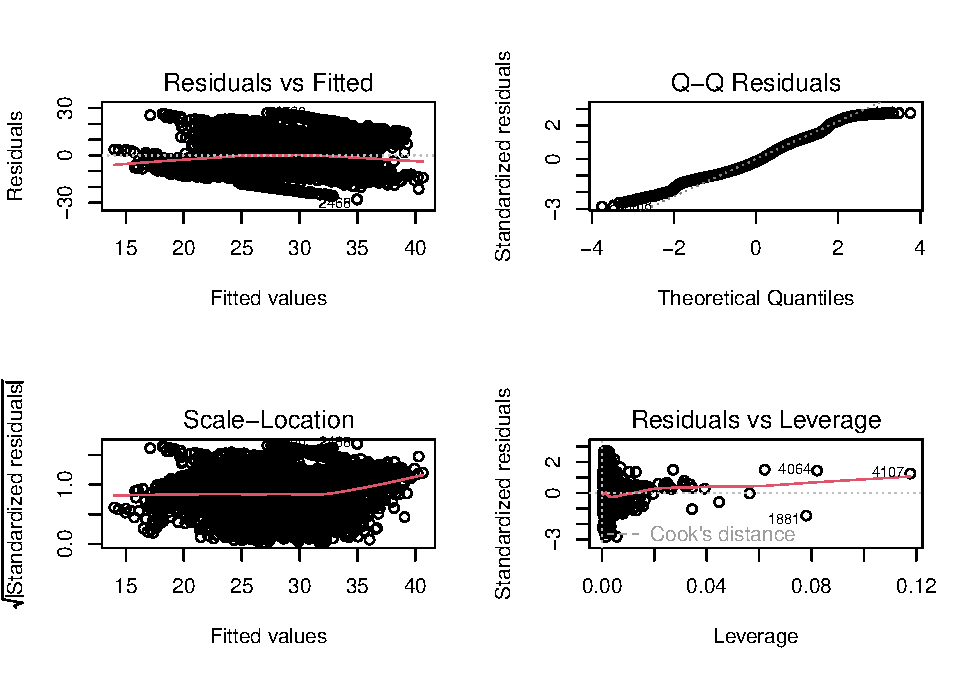
\includegraphics{Regression_files/figure-latex/unnamed-chunk-4-1.pdf}

\begin{Shaded}
\begin{Highlighting}[]
\FunctionTok{library}\NormalTok{(ggfortify)}
\FunctionTok{autoplot}\NormalTok{(mod1) }\SpecialCharTok{+} 
  \FunctionTok{theme\_bw}\NormalTok{()}
\end{Highlighting}
\end{Shaded}

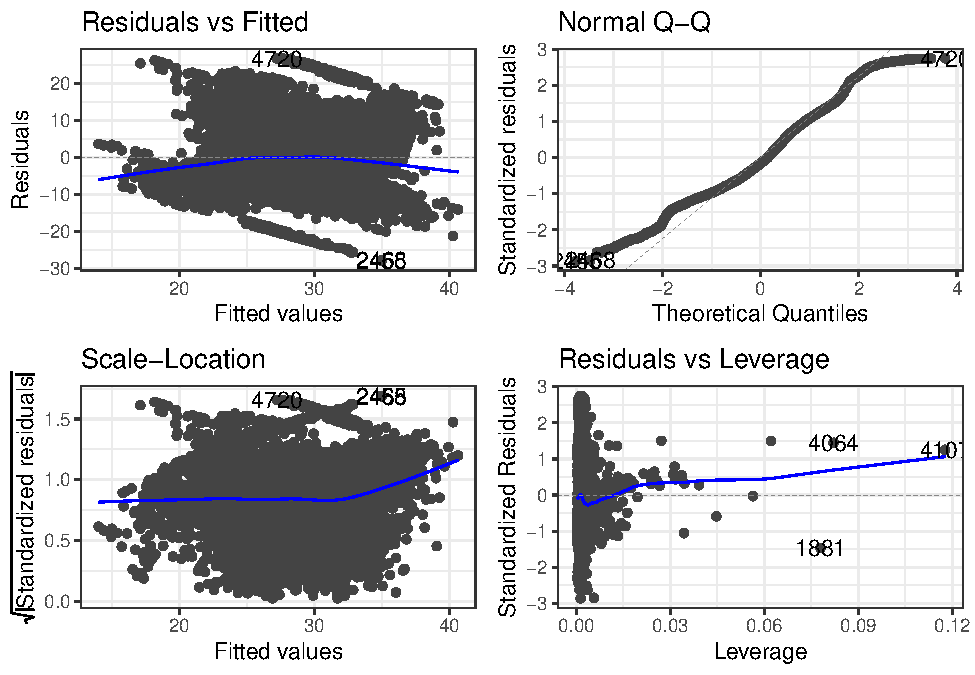
\includegraphics{Regression_files/figure-latex/unnamed-chunk-5-1.pdf}

We can also look how good are our fitted values:

\begin{Shaded}
\begin{Highlighting}[]
\FunctionTok{ggplot}\NormalTok{() }\SpecialCharTok{+} 
  \FunctionTok{geom\_point}\NormalTok{(}\FunctionTok{aes}\NormalTok{(}\AttributeTok{x =} \FunctionTok{fitted}\NormalTok{(mod1), }\AttributeTok{y =}\NormalTok{ dat}\SpecialCharTok{$}\NormalTok{total\_UPDRS)) }\SpecialCharTok{+}
  \FunctionTok{theme\_bw}\NormalTok{()}
\end{Highlighting}
\end{Shaded}

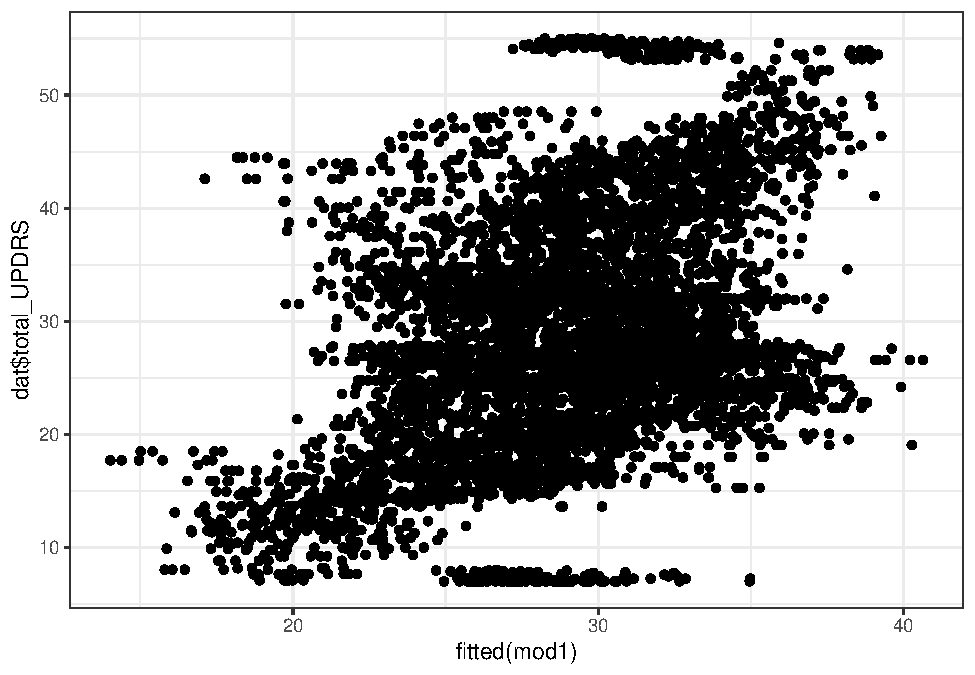
\includegraphics{Regression_files/figure-latex/unnamed-chunk-6-1.pdf}

It is clear that there is some peculiar behaviour. Let us try to
underline the observations belonging to each subject

\begin{Shaded}
\begin{Highlighting}[]
\FunctionTok{ggplot}\NormalTok{() }\SpecialCharTok{+} 
  \FunctionTok{geom\_abline}\NormalTok{(}\AttributeTok{linetype =} \StringTok{\textquotesingle{}dashed\textquotesingle{}}\NormalTok{) }\SpecialCharTok{+}
  \FunctionTok{geom\_point}\NormalTok{(}\FunctionTok{aes}\NormalTok{(}\AttributeTok{x =} \FunctionTok{fitted}\NormalTok{(mod1), }\AttributeTok{y =}\NormalTok{ dat}\SpecialCharTok{$}\NormalTok{total\_UPDRS, }\AttributeTok{col =}\NormalTok{ dat}\SpecialCharTok{$}\NormalTok{subject.)) }\SpecialCharTok{+} 
  \FunctionTok{theme\_bw}\NormalTok{()}
\end{Highlighting}
\end{Shaded}

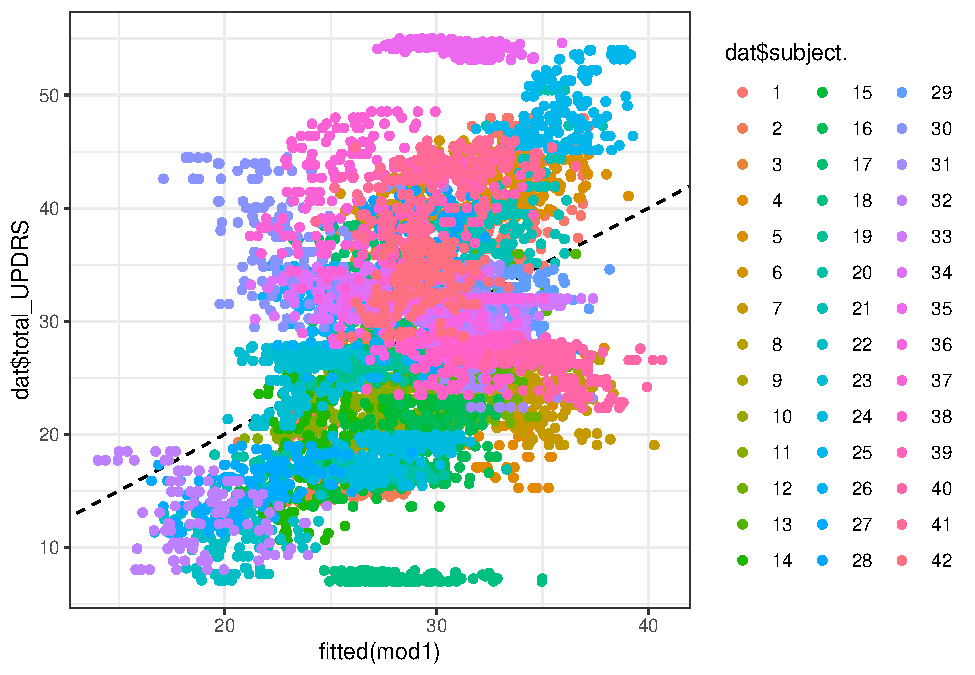
\includegraphics{Regression_files/figure-latex/unnamed-chunk-7-1.pdf}

It seems the response variable strongly depend on the subjects.

\hypertarget{assumptions}{%
\paragraph{Assumptions}\label{assumptions}}

\begin{enumerate}
\def\labelenumi{\arabic{enumi}.}
\tightlist
\item
  The errors in the regression should have conditional mean zero.
\item
  The regressors in \(X\) must all be linearly independent. Usually, it
  is also assumed that the regressors have finite moments up to at least
  the second moment. When this assumption is violated the regressors are
  called linearly dependent or perfectly multicollinear. In such case
  the value of the regression coefficient \(\beta\) cannot be learned.
\item
  Spherical errors, i.e.~\(Var[\epsilon|X] = \sigma^2 I_n\)
\item
  Errors are normally distributed.
  i.e.~\(\epsilon|X \sim N(0, \sigma^2 I_n)\).
\end{enumerate}

Let's focus on the residuals, and try to underline the errors belonging
to each subject.

\begin{Shaded}
\begin{Highlighting}[]
\FunctionTok{ggplot}\NormalTok{() }\SpecialCharTok{+} 
  \FunctionTok{geom\_abline}\NormalTok{(}\AttributeTok{intercept =} \DecValTok{0}\NormalTok{, }\AttributeTok{slope =} \DecValTok{0}\NormalTok{, }\AttributeTok{linetype =} \StringTok{\textquotesingle{}dashed\textquotesingle{}}\NormalTok{) }\SpecialCharTok{+}
  \FunctionTok{geom\_point}\NormalTok{(}\FunctionTok{aes}\NormalTok{(}\AttributeTok{x =} \FunctionTok{fitted}\NormalTok{(mod1), }\AttributeTok{y =} \FunctionTok{residuals}\NormalTok{(mod1), }\AttributeTok{col =}\NormalTok{ dat}\SpecialCharTok{$}\NormalTok{subject.)) }\SpecialCharTok{+} 
  \FunctionTok{theme\_bw}\NormalTok{()}
\end{Highlighting}
\end{Shaded}

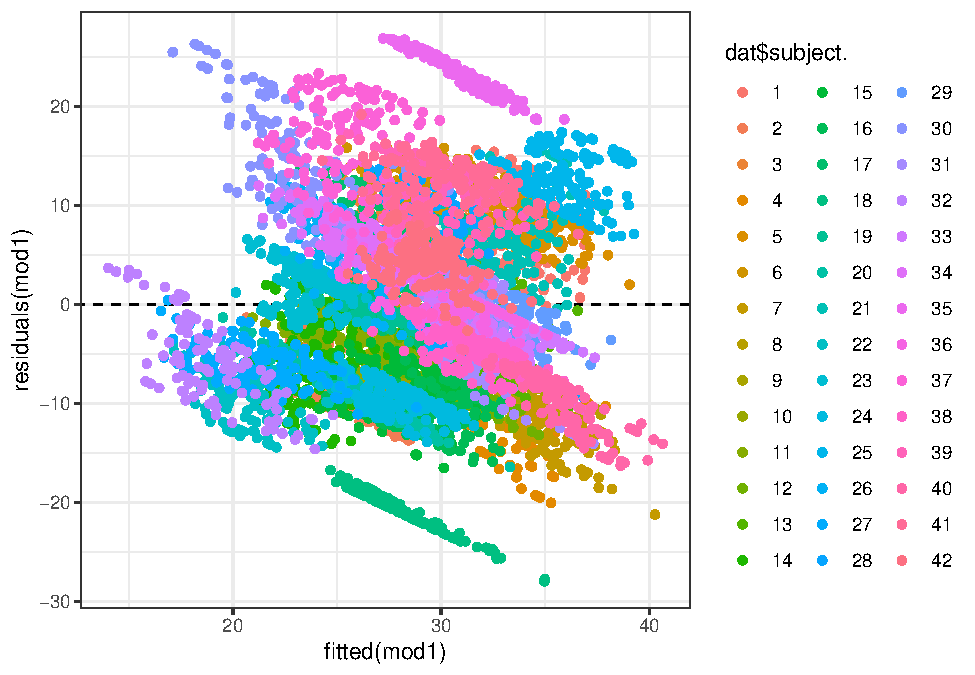
\includegraphics{Regression_files/figure-latex/unnamed-chunk-8-1.pdf}

We see that the residuals corresponding to the observations of a
specific subject are grouped together. This is a particular case in
which there is autocorrelation between residuals. In fact, since we have
repeated measures for each subject, it is not strange to imagine that
the errors belonging to a particular subject might be correlated. For
instance, imagine each subject having a different instrument, each
characterized by small measurement error. In this case, the observations
repeated observations taken by the subjects would be independent from
each other, but highly correlated within subject. Notice that the
distribution of estimates is much more spread out, with the variance
being higher, if correlated covariates are considered.

We can try to include the variable subject as a categorical variable

\begin{Shaded}
\begin{Highlighting}[]
\NormalTok{mod2 }\OtherTok{\textless{}{-}} \FunctionTok{lm}\NormalTok{(total\_UPDRS }\SpecialCharTok{\textasciitilde{}}\NormalTok{ subject. }\SpecialCharTok{+}\NormalTok{ age }\SpecialCharTok{+}\NormalTok{ sex }\SpecialCharTok{+}\NormalTok{ test\_time }\SpecialCharTok{+}
\NormalTok{             Jitter... }\SpecialCharTok{+}\NormalTok{ Shimmer }\SpecialCharTok{+}\NormalTok{ NHR }\SpecialCharTok{+}\NormalTok{ HNR }\SpecialCharTok{+}\NormalTok{ RPDE }\SpecialCharTok{+}\NormalTok{DFA }\SpecialCharTok{+}\NormalTok{ PPE,}
           \AttributeTok{data =}\NormalTok{ dat) }
\FunctionTok{summary}\NormalTok{(mod2)}
\end{Highlighting}
\end{Shaded}

\begin{verbatim}
## 
## Call:
## lm(formula = total_UPDRS ~ subject. + age + sex + test_time + 
##     Jitter... + Shimmer + NHR + HNR + RPDE + DFA + PPE, data = dat)
## 
## Residuals:
##     Min      1Q  Median      3Q     Max 
## -10.764  -1.257   0.037   1.506   9.248 
## 
## Coefficients: (2 not defined because of singularities)
##               Estimate Std. Error  t value Pr(>|t|)    
## (Intercept)  3.790e+01  1.097e+00   34.562  < 2e-16 ***
## subject.2   -2.417e+01  3.662e-01  -65.985  < 2e-16 ***
## subject.3   -7.340e+00  3.041e-01  -24.138  < 2e-16 ***
## subject.4   -1.682e+01  3.364e-01  -49.981  < 2e-16 ***
## subject.5    1.485e+00  3.148e-01    4.717 2.45e-06 ***
## subject.6    7.710e-01  3.125e-01    2.467  0.01364 *  
## subject.7   -1.742e+01  3.060e-01  -56.920  < 2e-16 ***
## subject.8   -1.476e+01  3.136e-01  -47.056  < 2e-16 ***
## subject.9   -1.569e+01  3.620e-01  -43.345  < 2e-16 ***
## subject.10  -2.092e+01  3.153e-01  -66.352  < 2e-16 ***
## subject.11  -1.781e+01  3.160e-01  -56.357  < 2e-16 ***
## subject.12  -1.629e+01  3.372e-01  -48.301  < 2e-16 ***
## subject.13  -1.273e+01  3.307e-01  -38.499  < 2e-16 ***
## subject.14  -2.272e+01  3.200e-01  -71.009  < 2e-16 ***
## subject.15  -2.151e+01  3.146e-01  -68.374  < 2e-16 ***
## subject.16  -2.183e+01  3.428e-01  -63.677  < 2e-16 ***
## subject.17  -8.845e+00  3.129e-01  -28.267  < 2e-16 ***
## subject.18  -3.321e+01  3.245e-01 -102.339  < 2e-16 ***
## subject.19  -1.477e+01  3.531e-01  -41.829  < 2e-16 ***
## subject.20  -2.371e+01  3.774e-01  -62.834  < 2e-16 ***
## subject.21  -2.733e-01  3.375e-01   -0.810  0.41807    
## subject.22  -2.994e+01  3.453e-01  -86.712  < 2e-16 ***
## subject.23  -1.521e+01  3.401e-01  -44.732  < 2e-16 ***
## subject.24  -2.204e+01  3.736e-01  -58.992  < 2e-16 ***
## subject.25   8.333e+00  3.164e-01   26.339  < 2e-16 ***
## subject.26  -9.101e+00  3.547e-01  -25.658  < 2e-16 ***
## subject.27  -2.538e+01  3.607e-01  -70.361  < 2e-16 ***
## subject.28  -5.586e+00  3.631e-01  -15.383  < 2e-16 ***
## subject.29  -9.504e+00  3.027e-01  -31.394  < 2e-16 ***
## subject.30  -3.618e+00  3.661e-01   -9.883  < 2e-16 ***
## subject.31  -1.129e+01  3.865e-01  -29.215  < 2e-16 ***
## subject.32  -2.745e+01  3.428e-01  -80.079  < 2e-16 ***
## subject.33  -9.971e+00  3.280e-01  -30.401  < 2e-16 ***
## subject.34  -8.064e+00  3.541e-01  -22.772  < 2e-16 ***
## subject.35   1.361e+01  3.412e-01   39.892  < 2e-16 ***
## subject.36  -9.013e+00  4.527e-01  -19.909  < 2e-16 ***
## subject.37   1.019e+00  3.192e-01    3.191  0.00142 ** 
## subject.38  -1.380e+01  3.119e-01  -44.265  < 2e-16 ***
## subject.39  -3.464e-01  3.102e-01   -1.117  0.26425    
## subject.40  -1.457e+01  3.180e-01  -45.819  < 2e-16 ***
## subject.41   2.074e+00  3.234e-01    6.413 1.54e-10 ***
## subject.42  -7.225e+00  3.074e-01  -23.504  < 2e-16 ***
## age                 NA         NA       NA       NA    
## sexM                NA         NA       NA       NA    
## test_time    1.872e-02  6.395e-04   29.270  < 2e-16 ***
## Jitter...    4.627e+01  1.485e+01    3.116  0.00184 ** 
## Shimmer      8.267e-01  3.059e+00    0.270  0.78698    
## NHR         -3.741e+00  1.683e+00   -2.223  0.02623 *  
## HNR          5.443e-02  2.304e-02    2.362  0.01820 *  
## RPDE        -1.040e-01  5.742e-01   -0.181  0.85624    
## DFA         -5.524e-01  1.093e+00   -0.505  0.61323    
## PPE         -8.488e-02  8.135e-01   -0.104  0.91690    
## ---
## Signif. codes:  0 '***' 0.001 '**' 0.01 '*' 0.05 '.' 0.1 ' ' 1
## 
## Residual standard error: 2.581 on 5825 degrees of freedom
## Multiple R-squared:  0.9423, Adjusted R-squared:  0.9418 
## F-statistic:  1941 on 49 and 5825 DF,  p-value: < 2.2e-16
\end{verbatim}

\begin{Shaded}
\begin{Highlighting}[]
\FunctionTok{ggplot}\NormalTok{(dat) }\SpecialCharTok{+} 
  \FunctionTok{geom\_point}\NormalTok{(}\FunctionTok{aes}\NormalTok{(}\AttributeTok{x =} \FunctionTok{fitted}\NormalTok{(mod2), }\AttributeTok{y =}\NormalTok{ total\_UPDRS, }\AttributeTok{color=}\NormalTok{subject.)) }\SpecialCharTok{+}
  \FunctionTok{geom\_abline}\NormalTok{(}\AttributeTok{linetype =} \StringTok{\textquotesingle{}dashed\textquotesingle{}}\NormalTok{) }
\end{Highlighting}
\end{Shaded}

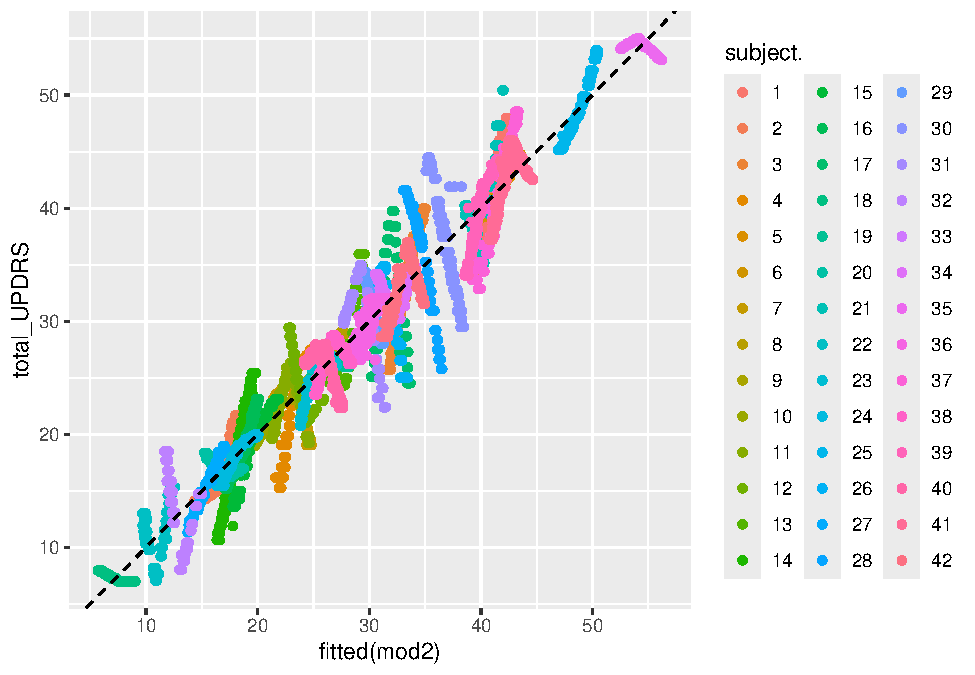
\includegraphics{Regression_files/figure-latex/unnamed-chunk-10-1.pdf}

Why R gives the warning (2 not defined because of singularities) and we
have two coefficients estimated as NA?

The problem is that we are including both an intercept and a number of
dummy variables equal to the number of patients. Let's try to visualize
this issue.

\begin{Shaded}
\begin{Highlighting}[]
\FunctionTok{library}\NormalTok{(reshape2)}
\NormalTok{mat }\OtherTok{\textless{}{-}} \FunctionTok{model.matrix}\NormalTok{(}\SpecialCharTok{\textasciitilde{}} \DecValTok{1} \SpecialCharTok{+}\NormalTok{ subject., }\AttributeTok{data =}\NormalTok{ dat)}
\NormalTok{dat\_mat }\OtherTok{\textless{}{-}} \FunctionTok{melt}\NormalTok{(mat)}
\FunctionTok{ggplot}\NormalTok{(dat\_mat, }\FunctionTok{aes}\NormalTok{(}\AttributeTok{x =}\NormalTok{ Var1, }\AttributeTok{y =}\NormalTok{ Var2, }\AttributeTok{fill =} \FunctionTok{as.factor}\NormalTok{(value))) }\SpecialCharTok{+} 
  \FunctionTok{geom\_tile}\NormalTok{() }\SpecialCharTok{+} 
  \FunctionTok{theme\_minimal}\NormalTok{()}
\end{Highlighting}
\end{Shaded}

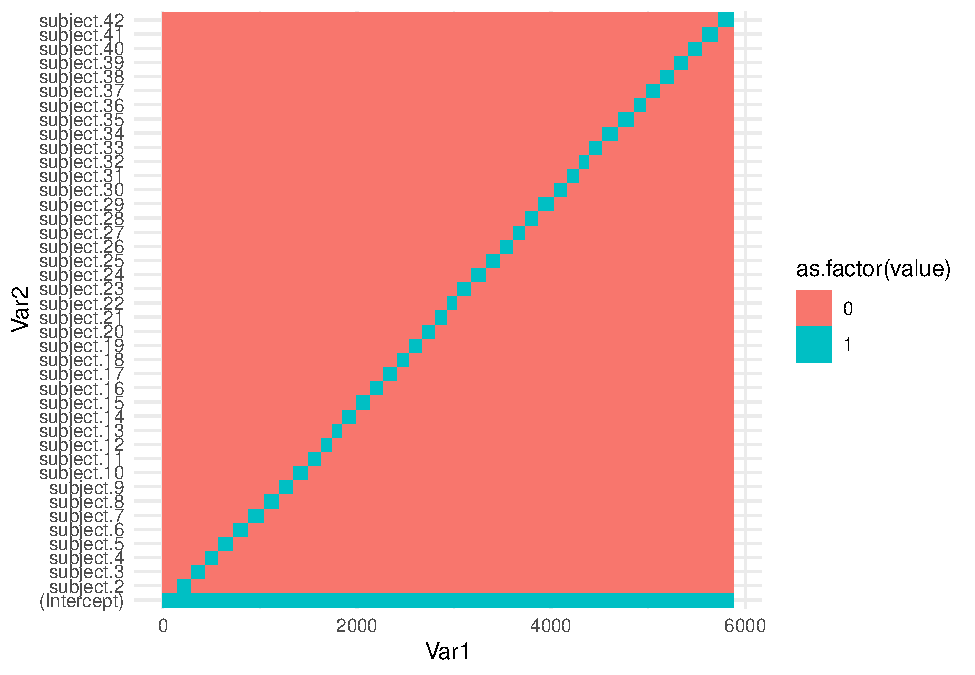
\includegraphics{Regression_files/figure-latex/unnamed-chunk-11-1.pdf}

Here we have perfect collinearity, since the intercept can be written as
a sum of all the dummy variables corresponding to subjects.

It is useful to consider estimation techniques for linear regressions
different from the classical least squares. One alternative id the
\emph{Iterative Reweighted Least Squares} (IRLS) which is commonly used
for robust regression or for generalized linear models. The MASS package
provides the \texttt{rlm} function for robust regression using IRLS.

\begin{Shaded}
\begin{Highlighting}[]
\FunctionTok{library}\NormalTok{(MASS)}
\NormalTok{model\_irls }\OtherTok{\textless{}{-}} \FunctionTok{rlm}\NormalTok{(total\_UPDRS }\SpecialCharTok{\textasciitilde{}}\NormalTok{  age }\SpecialCharTok{+}\NormalTok{ sex }\SpecialCharTok{+}\NormalTok{ test\_time }\SpecialCharTok{+}
\NormalTok{             Jitter... }\SpecialCharTok{+}\NormalTok{ Shimmer }\SpecialCharTok{+}\NormalTok{ NHR }\SpecialCharTok{+}\NormalTok{ HNR }\SpecialCharTok{+}\NormalTok{ RPDE }\SpecialCharTok{+}\NormalTok{ DFA }\SpecialCharTok{+}\NormalTok{ PPE,}
           \AttributeTok{data =}\NormalTok{ dat)}
\FunctionTok{summary}\NormalTok{(model\_irls)}
\end{Highlighting}
\end{Shaded}

\begin{verbatim}
## 
## Call: rlm(formula = total_UPDRS ~ age + sex + test_time + Jitter... + 
##     Shimmer + NHR + HNR + RPDE + DFA + PPE, data = dat)
## Residuals:
##     Min      1Q  Median      3Q     Max 
## -27.761  -7.179  -1.237   7.470  28.142 
## 
## Coefficients:
##             Value    Std. Error t value 
## (Intercept)  38.3448   3.0577    12.5402
## age           0.3029   0.0149    20.3232
## sexM          1.8840   0.2900     6.4953
## test_time     0.0154   0.0024     6.4990
## Jitter...   152.8948  49.5453     3.0860
## Shimmer     -43.7958  10.0786    -4.3454
## NHR         -23.2111   5.0831    -4.5663
## HNR          -0.5296   0.0670    -7.9057
## RPDE          6.4223   1.7360     3.6995
## DFA         -38.4485   2.1974   -17.4971
## PPE          11.2060   2.5814     4.3410
## 
## Residual standard error: 10.8 on 5864 degrees of freedom
\end{verbatim}

Another method is the \emph{Least Absolute Shrinkage and Selection
Operator} (LASSO), which can be performed using the \texttt{glmnet}
package.

\begin{Shaded}
\begin{Highlighting}[]
\FunctionTok{library}\NormalTok{(glmnet)}
\NormalTok{x\_matrix }\OtherTok{\textless{}{-}} \FunctionTok{as.matrix}\NormalTok{(dat[, }\FunctionTok{c}\NormalTok{(}\DecValTok{2}\SpecialCharTok{:}\DecValTok{4}\NormalTok{,}\DecValTok{7}\NormalTok{, }\DecValTok{12}\NormalTok{, }\DecValTok{18}\SpecialCharTok{:}\DecValTok{22}\NormalTok{)])}
\CommentTok{\# LASSO regression}
\NormalTok{model\_lasso }\OtherTok{\textless{}{-}} \FunctionTok{glmnet}\NormalTok{(x\_matrix, dat}\SpecialCharTok{$}\NormalTok{total\_UPDRS, }\AttributeTok{alpha =} \DecValTok{1}\NormalTok{)  }

\CommentTok{\# Cross{-}validation for selecting lambda}
\NormalTok{cv\_model }\OtherTok{\textless{}{-}} \FunctionTok{cv.glmnet}\NormalTok{(x\_matrix, dat}\SpecialCharTok{$}\NormalTok{total\_UPDRS, }\AttributeTok{alpha =} \DecValTok{1}\NormalTok{)}

\CommentTok{\# Best lambda}
\NormalTok{best\_lambda }\OtherTok{\textless{}{-}}\NormalTok{ cv\_model}\SpecialCharTok{$}\NormalTok{lambda.min}

\CommentTok{\# Model with the best lambda}
\NormalTok{model\_lasso\_best }\OtherTok{\textless{}{-}} \FunctionTok{glmnet}\NormalTok{(x\_matrix, dat}\SpecialCharTok{$}\NormalTok{total\_UPDRS, }\AttributeTok{alpha =} \DecValTok{1}\NormalTok{, }\AttributeTok{lambda =}\NormalTok{ best\_lambda)}
\FunctionTok{coef}\NormalTok{(model\_lasso\_best)}
\end{Highlighting}
\end{Shaded}

\begin{verbatim}
## 11 x 1 sparse Matrix of class "dgCMatrix"
##                       s0
## (Intercept)  35.87444701
## age           0.31019263
## sex           .         
## test_time     0.01560369
## Jitter...   105.51655615
## Shimmer     -37.11045108
## NHR         -27.57307268
## HNR          -0.53970963
## RPDE          5.28699135
## DFA         -32.33834432
## PPE          13.91418118
\end{verbatim}

The Bayesian information criterion (BIC) and Akaike information
criterion (AIC) offer a framework of comparing fits of models with a
different number of parameters.

\begin{Shaded}
\begin{Highlighting}[]
\CommentTok{\# AIC and BIC for LS}
\NormalTok{aic\_ls }\OtherTok{\textless{}{-}} \FunctionTok{AIC}\NormalTok{(mod1)}
\NormalTok{bic\_ls }\OtherTok{\textless{}{-}} \FunctionTok{BIC}\NormalTok{(mod1)}

\CommentTok{\# AIC and BIC for IRLS}
\NormalTok{n }\OtherTok{\textless{}{-}} \FunctionTok{length}\NormalTok{(dat}\SpecialCharTok{$}\NormalTok{total\_UPDRS)}
\NormalTok{logLik\_irls }\OtherTok{\textless{}{-}} \FunctionTok{sum}\NormalTok{(}\FunctionTok{dnorm}\NormalTok{(model\_irls}\SpecialCharTok{$}\NormalTok{residuals, }\AttributeTok{mean =} \DecValTok{0}\NormalTok{, }\AttributeTok{sd =} \FunctionTok{sd}\NormalTok{(model\_irls}\SpecialCharTok{$}\NormalTok{residuals), }\AttributeTok{log =} \ConstantTok{TRUE}\NormalTok{))}
\NormalTok{aic\_irls }\OtherTok{\textless{}{-}} \SpecialCharTok{{-}}\DecValTok{2} \SpecialCharTok{*}\NormalTok{ logLik\_irls }\SpecialCharTok{+} \DecValTok{2} \SpecialCharTok{*} \FunctionTok{length}\NormalTok{(}\FunctionTok{coef}\NormalTok{(model\_irls))}
\NormalTok{bic\_irls }\OtherTok{\textless{}{-}} \SpecialCharTok{{-}}\DecValTok{2} \SpecialCharTok{*}\NormalTok{ logLik\_irls }\SpecialCharTok{+} \FunctionTok{log}\NormalTok{(n) }\SpecialCharTok{*} \FunctionTok{length}\NormalTok{(}\FunctionTok{coef}\NormalTok{(model\_irls))}

\CommentTok{\# AIC and BIC for LASSO}
\NormalTok{y }\OtherTok{\textless{}{-}}\NormalTok{ dat}\SpecialCharTok{$}\NormalTok{total\_UPDRS}
\NormalTok{y\_hat\_lasso }\OtherTok{\textless{}{-}} \FunctionTok{predict}\NormalTok{(model\_lasso\_best, }\AttributeTok{s =}\NormalTok{ best\_lambda, }\AttributeTok{newx =} \FunctionTok{as.matrix}\NormalTok{(x\_matrix))}
\end{Highlighting}
\end{Shaded}

\begin{verbatim}
## Warning in cbind2(1, newx) %*% nbeta: NA introdotti per coercizione
\end{verbatim}

\begin{Shaded}
\begin{Highlighting}[]
\NormalTok{rss\_lasso }\OtherTok{\textless{}{-}} \FunctionTok{sum}\NormalTok{((y }\SpecialCharTok{{-}}\NormalTok{ y\_hat\_lasso)}\SpecialCharTok{\^{}}\DecValTok{2}\NormalTok{)}
\NormalTok{sigma\_hat\_lasso }\OtherTok{\textless{}{-}} \FunctionTok{sqrt}\NormalTok{(rss\_lasso }\SpecialCharTok{/}\NormalTok{ n)}
\NormalTok{logLik\_lasso }\OtherTok{\textless{}{-}} \SpecialCharTok{{-}}\NormalTok{n }\SpecialCharTok{/} \DecValTok{2} \SpecialCharTok{*} \FunctionTok{log}\NormalTok{(}\DecValTok{2} \SpecialCharTok{*}\NormalTok{ pi }\SpecialCharTok{*}\NormalTok{ sigma\_hat\_lasso}\SpecialCharTok{\^{}}\DecValTok{2}\NormalTok{) }\SpecialCharTok{{-}}\NormalTok{ rss\_lasso }\SpecialCharTok{/}\NormalTok{ (}\DecValTok{2} \SpecialCharTok{*}\NormalTok{ sigma\_hat\_lasso}\SpecialCharTok{\^{}}\DecValTok{2}\NormalTok{)}
\NormalTok{aic\_lasso }\OtherTok{\textless{}{-}} \SpecialCharTok{{-}}\DecValTok{2} \SpecialCharTok{*}\NormalTok{ logLik\_lasso }\SpecialCharTok{+} \DecValTok{2} \SpecialCharTok{*} \FunctionTok{sum}\NormalTok{(}\FunctionTok{coef}\NormalTok{(model\_lasso\_best) }\SpecialCharTok{!=} \DecValTok{0}\NormalTok{)}
\NormalTok{bic\_lasso }\OtherTok{\textless{}{-}} \SpecialCharTok{{-}}\DecValTok{2} \SpecialCharTok{*}\NormalTok{ logLik\_lasso }\SpecialCharTok{+} \FunctionTok{log}\NormalTok{(n) }\SpecialCharTok{*} \FunctionTok{sum}\NormalTok{(}\FunctionTok{coef}\NormalTok{(model\_lasso\_best) }\SpecialCharTok{!=} \DecValTok{0}\NormalTok{)}

\CommentTok{\# Combine Results}
\NormalTok{comparison }\OtherTok{\textless{}{-}} \FunctionTok{data.frame}\NormalTok{(}
  \AttributeTok{Model =} \FunctionTok{c}\NormalTok{(}\StringTok{"LS"}\NormalTok{, }\StringTok{"IRLS"}\NormalTok{, }\StringTok{"LASSO"}\NormalTok{),}
  \AttributeTok{AIC =} \FunctionTok{c}\NormalTok{(aic\_ls, aic\_irls, aic\_lasso),}
  \AttributeTok{BIC =} \FunctionTok{c}\NormalTok{(bic\_ls, bic\_irls, bic\_lasso)}
\NormalTok{)}
\FunctionTok{print}\NormalTok{(comparison)}
\end{Highlighting}
\end{Shaded}

\begin{verbatim}
##   Model      AIC      BIC
## 1    LS 43493.74 43573.88
## 2  IRLS 43508.98 43582.44
## 3 LASSO 43531.50 43598.29
\end{verbatim}

We finally construct a table comparing the obtained estimates

\begin{Shaded}
\begin{Highlighting}[]
\NormalTok{coeff\_ls }\OtherTok{\textless{}{-}} \FunctionTok{coef}\NormalTok{(mod1)}
\NormalTok{coeff\_irls }\OtherTok{\textless{}{-}} \FunctionTok{coef}\NormalTok{(model\_irls)}
\NormalTok{coeff\_lasso }\OtherTok{\textless{}{-}} \FunctionTok{coef}\NormalTok{(model\_lasso\_best)[}\SpecialCharTok{{-}}\DecValTok{1}\NormalTok{]  }\CommentTok{\# Remove intercept for comparison}

\CommentTok{\# Combine Results}
\NormalTok{coefficients }\OtherTok{\textless{}{-}} \FunctionTok{data.frame}\NormalTok{(}
  \AttributeTok{Variable =} \FunctionTok{c}\NormalTok{(}\StringTok{"(Intercept)"}\NormalTok{, }\FunctionTok{paste0}\NormalTok{(}\StringTok{"X"}\NormalTok{, }\DecValTok{1}\SpecialCharTok{:}\DecValTok{10}\NormalTok{)),}
  \AttributeTok{LS =}\NormalTok{ coeff\_ls,}
  \AttributeTok{IRLS =}\NormalTok{ coeff\_irls,}
  \AttributeTok{LASSO =} \FunctionTok{c}\NormalTok{(}\FunctionTok{as.numeric}\NormalTok{(}\FunctionTok{coef}\NormalTok{(model\_lasso\_best)[}\DecValTok{1}\NormalTok{]), }\FunctionTok{as.numeric}\NormalTok{(coeff\_lasso)))}

\CommentTok{\# View Results}
\FunctionTok{print}\NormalTok{(coefficients)}
\end{Highlighting}
\end{Shaded}

\begin{verbatim}
##                Variable           LS         IRLS        LASSO
## (Intercept) (Intercept)  37.99303565  38.34480753  35.87444701
## age                  X1   0.30912518   0.30292540   0.31019263
## sexM                 X2   1.89536037   1.88397176   0.00000000
## test_time            X3   0.01560014   0.01541468   0.01560369
## Jitter...            X4 101.44342681 152.89484031 105.51655615
## Shimmer              X5 -42.26209151 -43.79583797 -37.11045108
## NHR                  X6 -22.39076525 -23.21113933 -27.57307268
## HNR                  X7  -0.58739500  -0.52957482  -0.53970963
## RPDE                 X8   3.08313516   6.42232561   5.28699135
## DFA                  X9 -33.41483563 -38.44852881 -32.33834432
## PPE                 X10  12.19349626  11.20598927  13.91418118
\end{verbatim}

\begin{Shaded}
\begin{Highlighting}[]
\CommentTok{\# Plotting Coefficients for Comparison}
\FunctionTok{library}\NormalTok{(reshape2)}
\NormalTok{coeff\_melt }\OtherTok{\textless{}{-}} \FunctionTok{melt}\NormalTok{(coefficients, }\AttributeTok{id.vars =} \StringTok{"Variable"}\NormalTok{, }\AttributeTok{variable.name =} \StringTok{"Method"}\NormalTok{, }\AttributeTok{value.name =} \StringTok{"Coefficient"}\NormalTok{)}

\FunctionTok{library}\NormalTok{(ggplot2)}
\FunctionTok{ggplot}\NormalTok{(coeff\_melt, }\FunctionTok{aes}\NormalTok{(}\AttributeTok{x =}\NormalTok{ Variable, }\AttributeTok{y =}\NormalTok{ Coefficient, }\AttributeTok{fill =}\NormalTok{ Method)) }\SpecialCharTok{+}
  \FunctionTok{geom\_bar}\NormalTok{(}\AttributeTok{stat =} \StringTok{"identity"}\NormalTok{, }\AttributeTok{position =} \StringTok{"dodge"}\NormalTok{) }\SpecialCharTok{+}
  \FunctionTok{theme\_minimal}\NormalTok{() }\SpecialCharTok{+}
  \FunctionTok{labs}\NormalTok{(}\AttributeTok{title =} \StringTok{"Comparison of Coefficients"}\NormalTok{, }\AttributeTok{y =} \StringTok{"Coefficient Estimate"}\NormalTok{, }\AttributeTok{x =} \StringTok{"Predictor Variable"}\NormalTok{)}
\end{Highlighting}
\end{Shaded}

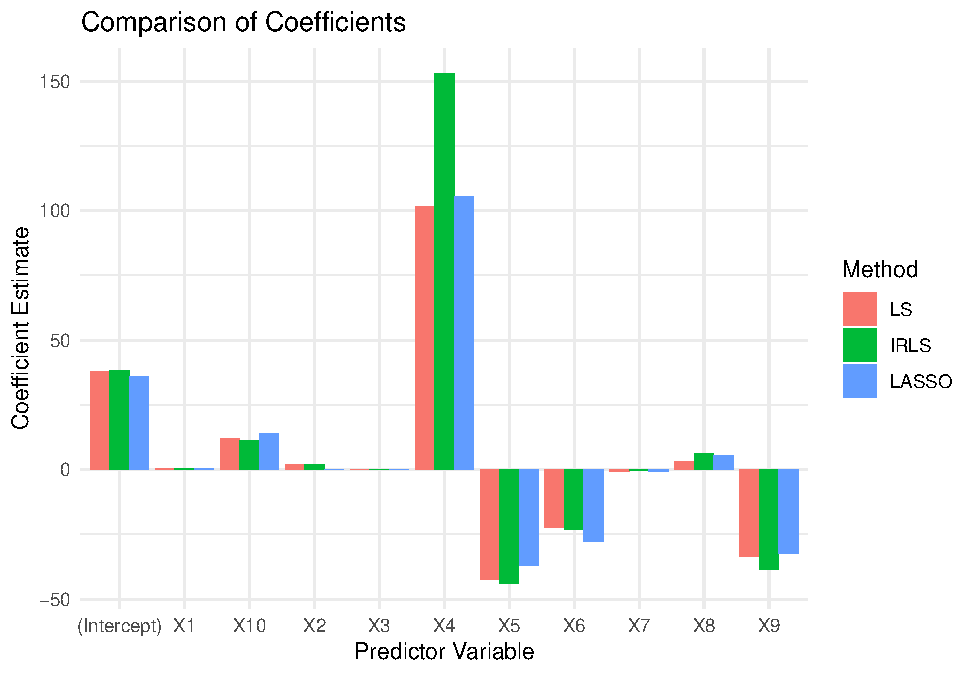
\includegraphics{Regression_files/figure-latex/unnamed-chunk-15-1.pdf}

\end{document}
